\documentclass[10pt]{article}
\usepackage[french]{babel}
\usepackage[utf8]{inputenc}
\usepackage[T1]{fontenc}
\usepackage{amsmath}
\usepackage{amsfonts}
\usepackage{amssymb}
\usepackage[version=4]{mhchem}
\usepackage{stmaryrd}
\usepackage{bbold}
\usepackage{graphicx}
\usepackage[export]{adjustbox}
\graphicspath{ {./images/} }
\usepackage{caption}

\title{TP1 Analyse numérique (B1-TP1) }

\author{Ibrahim ALAME}
\date{}


\begin{document}
\maketitle
\captionsetup{singlelinecheck=false}
3/04/2024

\section*{1 Problème de la chaleur}
Soit \(O L\) une barre chauffée initialement à la température \(\theta(x)=\sin ^{2}\left(2 \pi \frac{x}{L}\right), 0 \leq x \leq L\). On cherche à refroidir la barre en appliquant une température 0 aux extrémités \(O\) et \(L\). Déterminer l'évolution de la température \(u(x, t)\) en tout point \(x\) de la barre et à chaque instant \(t \geq 0\) :

\[
\begin{cases}\frac{\partial u}{\partial t}-\kappa \frac{\partial^{2} u}{\partial x^{2}}=0 & \forall(x, t) \in[0, L] \times \mathbb{R}^{+} \\ u(x, 0)=\theta(x) & \forall x \in[0, L] \\ u(0, t)=u(L, t)=0 & \forall t \in \mathbb{R}^{+}\end{cases}
\]

\begin{center}
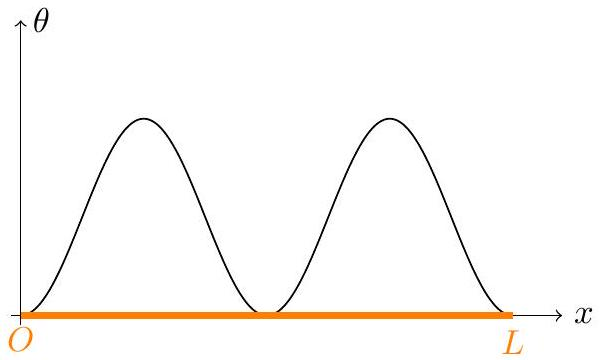
\includegraphics[max width=\textwidth, alt={}]{c96d1874-7092-4616-9726-d747c0247b13-1_360_603_1241_762}
\end{center}

On prendra \(\kappa=0.1, L=1\) et on choisira un pas de temps \(\tau=0.0005\)

\begin{verbatim}
# Initialisation des constantes
L=1; kappa = 0.1
h=0.01; tau= 0.0005
c = kappa * tau / h**2
\end{verbatim}

et on discrétisera l'intervalle \([0, L]\) en \(N\) sous-intervalles avec un pas \(h=0.01\) ( \(N+1\) points de discrétisation).

\begin{verbatim}
# Coordonnées en espace
N = int(L / h)
X = np.linspace(0, L, N+1)
\end{verbatim}

L'animation de l'évolution de la température est à afficher dans une fenêtre \(800 \times 600\) de la librairie python tkinter:

\begin{verbatim}
\#==========================================
fen1 \(=\mathrm{Tk}()\) \# Création de la fenêtre principale
fen1.title("Equation de la chaleur")
\(\mathrm{W}=800\); \(\mathrm{H}=600\)
\# Définir une zone graphique \(W \times H\)
can1 = Canvas(fen1,bg = 'dark gray', width \(=\mathrm{W}\), height \(=\mathrm{H}\) )
can1.pack() \# Positionne can1 dans la fenêtre fen1
DF() \# Fonction de calcul en Diff Finies et affichage graphique
fen1.mainloop() \# Boucle principale de la fenêtre
\end{verbatim}

où DF() est la fonction qui calcule et affiche la température de la barre à l'instant \(t_{n}=n \tau\) à partir du schéma de la méthode explicite :

\[
\frac{u_{i}^{n}-u_{i}^{n-1}}{\tau}-\kappa \frac{u_{i-1}^{n-1}-2 u_{i}^{n-1}+u_{i+1}^{n-1}}{h^{2}}=0
\]

\begin{verbatim}
def DF():
    global UO \# on désigne par UO[i] la solution à l'instant précédent \(u\left(x_{i}, t_{n-1}\right)=u_{i}^{n-1}\)
    can1.delete('all') \# on efface la courbe de l'instant t-1
    \(\mathrm{U}=n \mathrm{p} \cdot \operatorname{zeros}(\mathrm{N}+1) \# U[i]\) est la solution à l'instant actuel \(u\left(x_{i}, t_{n}\right)=u_{i}^{n}\)
    for i in range(1,N):
        \(\mathrm{U}[\mathrm{i}]=\ldots\)
    \# courbe à l'instant \(t\); segment entre deux points consécutifs: create_line \(\left(x_{i-1}, y_{i-1}, x_{i}, y_{i}\right)\)
    for i in range(1,N+1):
        can1.create_line \((\mathrm{X}[\mathrm{i}-1] * \mathrm{~W},(1-\mathrm{U}[\mathrm{i}-1]) * \mathrm{H} / 2, \mathrm{X}[\mathrm{i}] * \mathrm{~W},(1-\mathrm{U}[\mathrm{i}]) * \mathrm{H} / 2, \mathrm{fill}=\) 'blue', width=5)
    UO = U.copy()
    fen1.after(10, DF) \# réexécute la fonction \(D F()\) à l'instant suivant après 10 ms
\end{verbatim}

\[
\left\{\begin{array}{l}
x=X \cdot W \\
y=(1-Y) \cdot H / 2
\end{array}\right.
\]

\begin{figure}[h]
\begin{center}
\captionsetup{labelformat=empty}
\caption{Transformation géométrique entre le repère informatique ( \(O x y\) ) et le repère mathématique ( \(\Omega X Y\) )}
  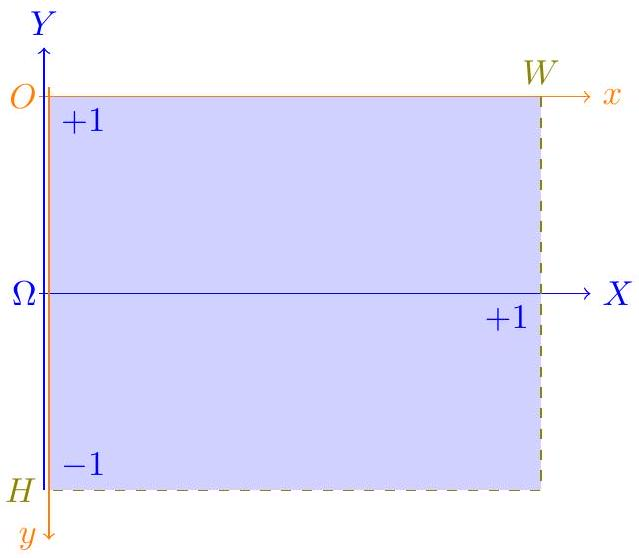
\includegraphics[alt={},max width=\textwidth]{c96d1874-7092-4616-9726-d747c0247b13-2_558_639_1533_1001}
\end{center}
\end{figure}

\section*{2 Propagation des ondes}
On considère une corde de masse linéïque \(\rho\) fixée en ses deux extrémités \(O\) et \(L\) et tendue avec une grande force \(F\). On pose \(c=\sqrt{\frac{F}{\rho}}\). A l'instant \(t=0\), on déplace verticalement chaque point d'abscisse \(x\) d'une distance \(f(x)\) à une vitesse initiale \(g(x)\). En petites perturbations, le déplacement \(u(x, t)\) en tout point \(x\) de la corde et à chaque instant \(t \geq 0\) est solution du problème des ondes suivant :

\[
\begin{cases}\frac{\partial^{2} u}{\partial t^{2}}-c^{2} \frac{\partial^{2} u}{\partial x^{2}}=0 & \forall(x, t) \in[0, L] \times \mathbb{R}^{+} \\ u(x, 0)=f(x) & \forall x \in[0, L] \\ \frac{\partial u}{\partial t}(x, 0)=g(x) & \forall x \in[0, L] \\ u(0, t)=u(L, t)=0 & \forall t \in \mathbb{R}^{+}\end{cases}
\]

Résoudre numériquement ce problème par la méthode des différences finies :

\[
\frac{u_{i}^{n}-2 u_{i}^{n-1}+u_{i}^{n-2}}{\tau^{2}}-c^{2} \frac{u_{i+1}^{n-1}-2 u_{i}^{n-1}+u_{i-1}^{n-1}}{h^{2}}=0
\]

en prenant les données numériques suivantes :

\[
h=0.01, \quad \tau=0.001, \quad L=1 \mathrm{~m}, \quad c=5 \mathrm{~m} / \mathrm{s}, \quad f(x)=e^{-500(x-L / 2)^{2}}, \quad g(x)=0
\]

afficher le résultat en animation graphique dans une fenêtre tkinter de hauteur \(H=800 \mathrm{px}\) et de largeur \(W=800 \mathrm{px}\).

\section*{3 Équation de diffusion}
On considère l'équation d'advection suivante :

\[
\left\{\begin{array}{l}
\frac{\partial u}{\partial t}+V \frac{\partial u}{\partial x}=0, \quad 0 \leq x \leq \ell, \quad t \in \mathbb{R}^{+} \\
u(x+\ell, t)=u(x, t) \\
u(x, 0)=u_{0}(x)=f(x)
\end{array}\right.
\]

On prendra \(\ell=1 \mathrm{~m}, \quad f(x)=0.9 e^{-100(x-\ell / 2)^{2}}, \quad V=3 \mathrm{~m} / \mathrm{s}, \quad h=0.005 \mathrm{~m}, \quad \tau=0.0002 \mathrm{~s}\)

\begin{enumerate}
  \item Pour résoudre ce problème, programmer le schéma explicite centré, suivants :
\end{enumerate}

\[
\frac{u_{i}^{n}-u_{i}^{n-1}}{\tau}+V \frac{u_{i+1}^{n-1}-u_{i-1}^{n-1}}{2 h}=0
\]

où \(u\) est un tableau de taille \(N=\operatorname{int}\left(\frac{\ell}{h}\right)\) (partie entière). \(u_{i}\) est donc défini pour \(i= 0,1, \cdots, N-1\). Le calcul de \(u_{0}\) et \(u_{N-1}\) nécessite les valeurs de \(u_{-1}\) et \(u_{N}\) et compte tenu de la périodicité on remplacera alors \(u_{N}\) par \(u_{0}\) et \(u_{-1}\) par \(u_{N-1}\).\\
2. Schéma de Lax-Wendroff On fait un développement limité à l'ordre 2 en temps de \(u(x, t)\) :

\[
u\left(x_{i}, t_{n+1}\right)=u\left(x_{i}, t_{n}\right)+\tau \frac{\partial u}{\partial t}\left(x_{i}, t_{n}\right)+\frac{\tau^{2}}{2} \frac{\partial^{2} u}{\partial t^{2}}\left(x_{i}, t_{n}\right)+o\left(\tau^{2}\right)
\]

Nous allons passer les dérivées partielles par rapport au temps à des dérivées partielles par rapport à l'espace :

\[
\frac{\partial u}{\partial t}=-V \frac{\partial u}{\partial x}
\]

et

\[
\frac{\partial^{2} u}{\partial t^{2}}=-V \frac{\partial}{\partial t}\left[\frac{\partial u}{\partial x}\right]=-V \frac{\partial}{\partial x}\left[\frac{\partial u}{\partial t}\right]=+V^{2} \frac{\partial^{2} u}{\partial x^{2}}
\]

Finalement

\[
u\left(x_{i}, t_{n+1}\right)=u\left(x_{i}, t_{n}\right)-\tau V \frac{\partial u}{\partial x}\left(x_{i}, t_{n}\right)+\frac{\tau^{2} V^{2}}{2} \frac{\partial^{2} u}{\partial x^{2}}\left(x_{i}, t_{n}\right)+o\left(\tau^{2}\right)
\]

D'où le schéma de Lax-Wendroff :

\[
\frac{u_{i}^{n}-u_{i}^{n-1}}{\tau}+V \frac{u_{i+1}^{n-1}-u_{i-1}^{n-1}}{2 h}-\frac{\tau V^{2}}{2} \frac{u_{i+1}^{n-1}-2 u_{i}^{n-1}+u_{i-1}^{n-1}}{h^{2}}=0
\]

Programmer ce schéma et comparer avec la méthode explicite centrée.


\end{document}